\documentclass{beamer}

\mode<presentation> {

%\usetheme{default}
%\usetheme{AnnArbor}
%\usetheme{Antibes}
%\usetheme{Bergen}
%\usetheme{Berkeley}
%\usetheme{Berlin}
%\usetheme{Boadilla}
%\usetheme{CambridgeUS}
%\usetheme{Copenhagen}
%\usetheme{Darmstadt}
%\usetheme{Dresden}
%\usetheme{Frankfurt}
%\usetheme{Goettingen}
%\usetheme{Hannover}
%\usetheme{Ilmenau}
%\usetheme{JuanLesPins}
%\usetheme{Luebeck}
\usetheme{Madrid}
%\usetheme{Malmoe}
%\usetheme{Marburg}
%\usetheme{Montpellier}
%\usetheme{PaloAlto}
%\usetheme{Pittsburgh}
%\usetheme{Rochester}
%\usetheme{Singapore}
%\usetheme{Szeged}
%\usetheme{Warsaw}


%\usecolortheme{albatross}
%\usecolortheme{beaver}
%\usecolortheme{beetle}
%\usecolortheme{crane}
%\usecolortheme{dolphin}
%\usecolortheme{dove}
%\usecolortheme{fly}
%\usecolortheme{lily}
%\usecolortheme{orchid}
%\usecolortheme{rose}
%\usecolortheme{seagull}
%\usecolortheme{seahorse}
%\usecolortheme{whale}
%\usecolortheme{wolverine}

%\setbeamertemplate{footline} % To remove the footer line in all slides uncomment this line
%\setbeamertemplate{footline}[page number] % To replace the footer line in all slides with a simple slide count uncomment this line

%\setbeamertemplate{navigation symbols}{} % To remove the navigation symbols from the bottom of all slides uncomment this line
}

\usepackage{graphicx} % Allows including images
\usepackage{booktabs} % Allows the use of \toprule, \midrule and \bottomrule in tables
\usepackage{amsfonts}
\usepackage{mathrsfs}
\usepackage{amsmath,amssymb,graphicx, bm}
\usepackage{dirtytalk} % quote thing

%----------------------------------------------------------------------------------------
%	TITLE PAGE
%----------------------------------------------------------------------------------------

\title["8.1"]{8.1: Multivariate Time Series Examples}

\author{Taylor} 
\institute[UVA] 
{
University of Virginia \\
\medskip
\textit{} 
}
\date{} 

\begin{document}
%----------------------------------------------------------------------------------------

\begin{frame}
\titlepage 
\end{frame}
%----------------------------------------------------------------------------------------

\begin{frame}
\frametitle{Motivation}

$\mathbf{X}_t$ is a vector-valued time series now. We usually consider the bivariate case for clarity, although most of what we learn will apply to higher dimensions.
\newline

Each time series $\{X_{t,1}\}$ and $\{X_{t,2}\}$ can be considered separately with the techniques we learned before. Although, this does not take into account the relationship they have between each other.
\end{frame}

%----------------------------------------------------------------------------------------

\begin{frame}
\frametitle{Motivation}

Weekly log-returns and their cumulative sums.
\begin{centering}
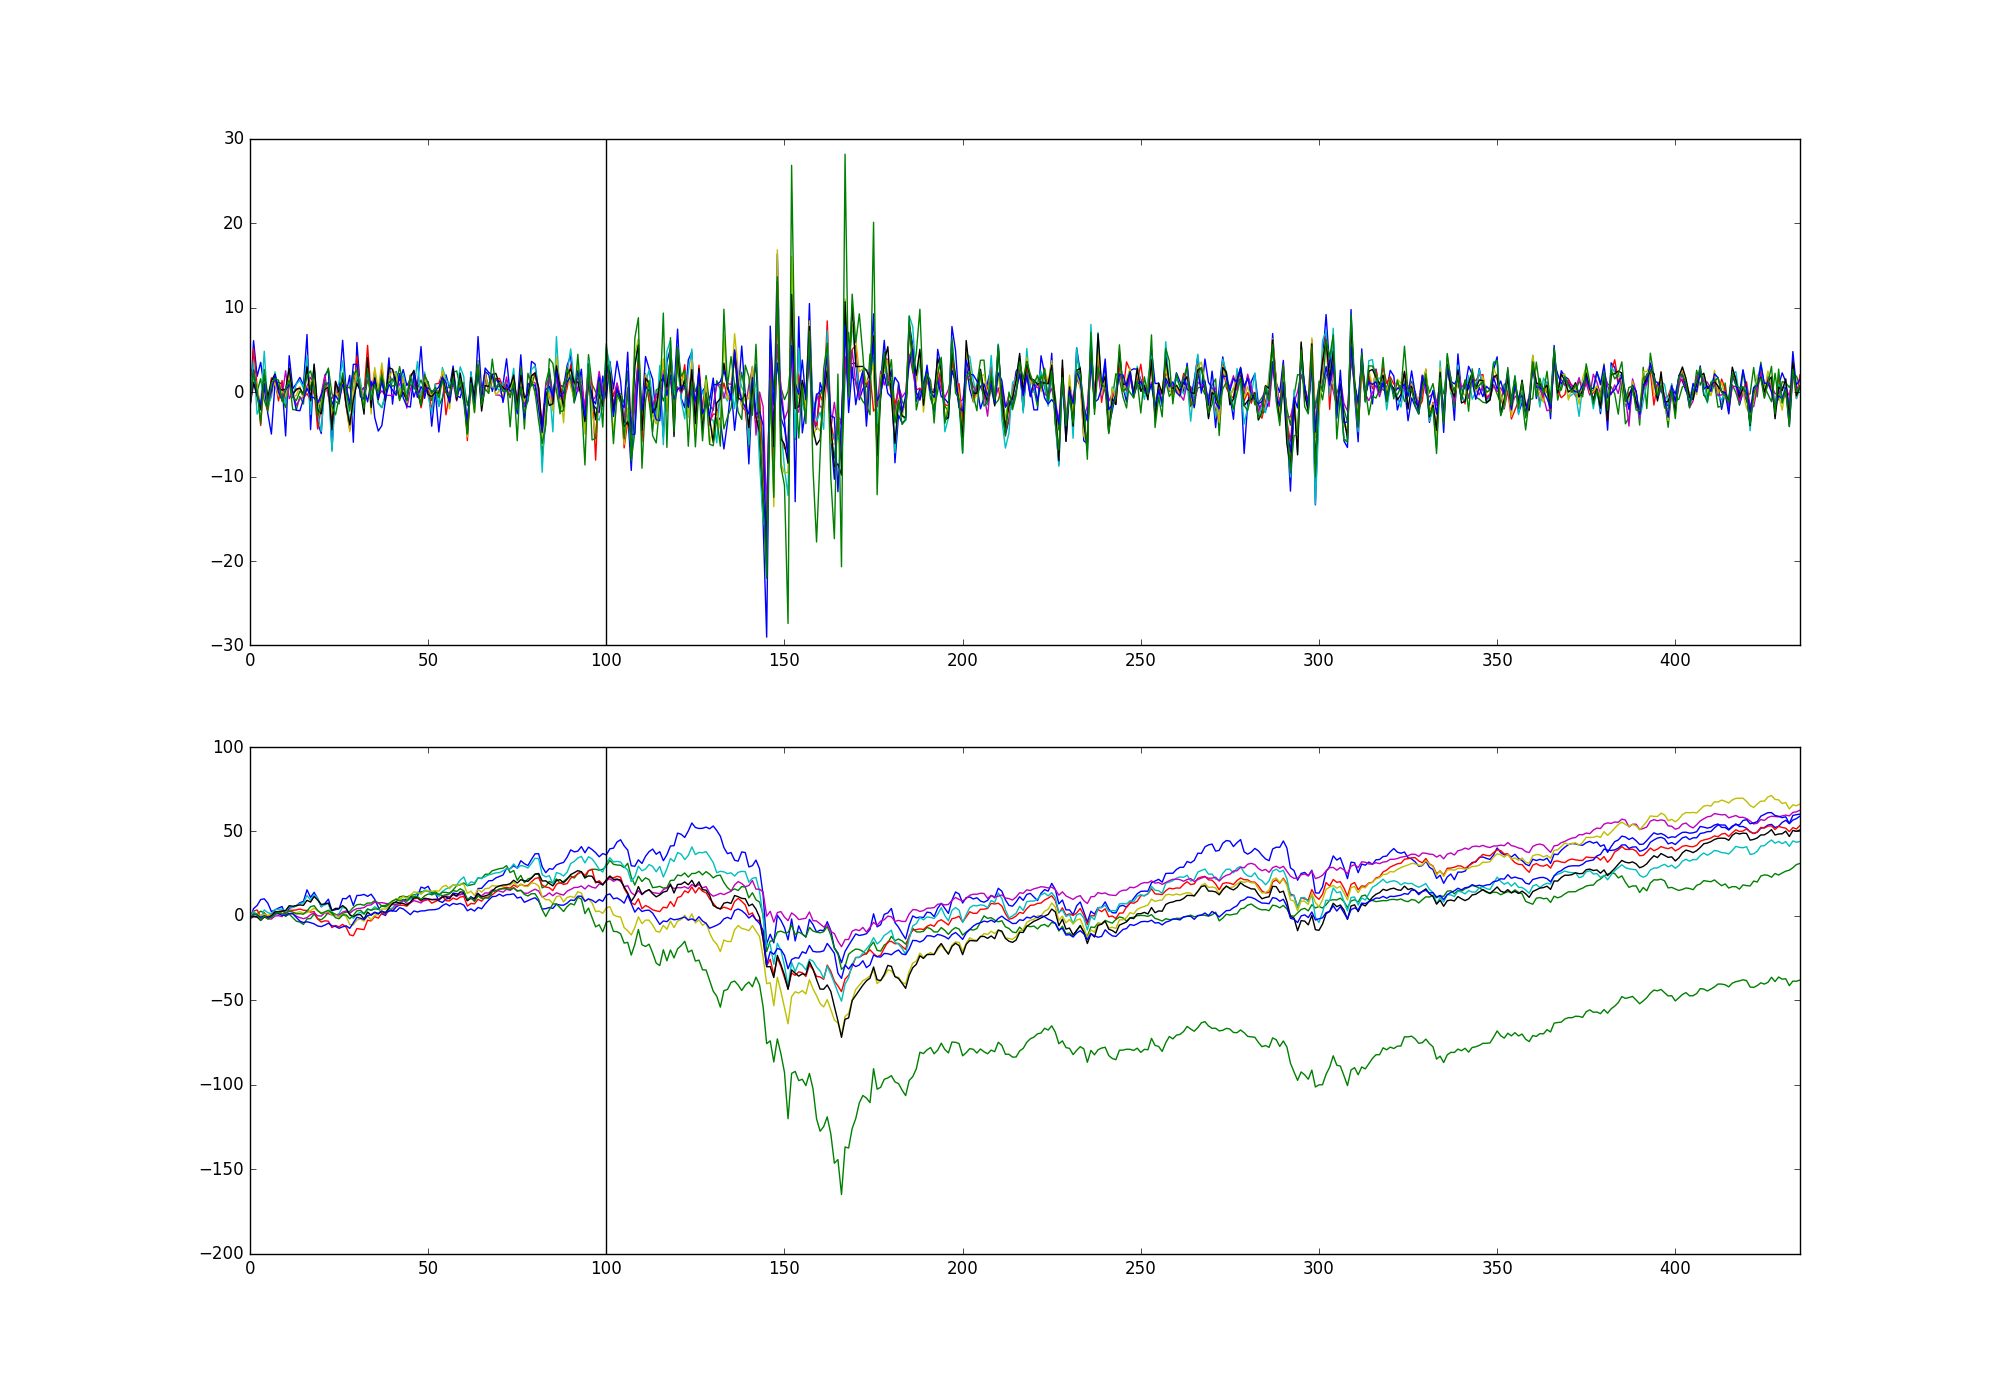
\includegraphics[width=100mm]{./pics/weekly_etfs.png}
\end{centering}
Select Sector SPDR ETFs 2005/12/23-2014/5/1. 


\end{frame}



%----------------------------------------------------------------------------------------

\begin{frame}
\frametitle{Means and Covariances}

The mean vector is
\[
\bm{\mu}_t = 
E[\mathbf{X}_t] =
\left[\begin{array}{c}
EX_{t,1} \\
EX_{t,2}
\end{array}\right]
\]
and the covariance matrices are
\[
\Gamma(t+h,t) = \text{Cov}(\mathbf{X}_{t+h},\mathbf{X}_t) = 
\left[\begin{array}{cc}
\text{Cov}(X_{t+h,1}, X_{t,1}) & \text{Cov}(X_{t+h,1}, X_{t,2}) \\
\text{Cov}(X_{t+h,2}, X_{t,1}) & \text{Cov}(X_{t+h,2}, X_{t,2})
\end{array}\right]
\]
for each $h$

\end{frame}

%----------------------------------------------------------------------------------------

\begin{frame}
\frametitle{Means and Covariances}

\begin{block}{weak stationarity}
A bivariate series $\mathbf{X}_t$ is said to be {\bf weakly stationary }if $\bm{\mu}_t$ and $\Gamma(t+h,t)$ are independent of $t$.
\end{block}

If that's the case, we will write $\bm{\mu}$ and $\Gamma(h)$ for these quantities. 
\newline

Notice that 
\[
\gamma_{12}(h) = \text{Cov}(X_{t+h,1},X_{t,2}) =\text{Cov}(X_{t,2}, X_{t+h,1})  = \gamma_{21}(-h)
\]
so these matrices are not symmetric!

\end{frame}
%----------------------------------------------------------------------------------------

\begin{frame}
\frametitle{Means and Covariances (and correlations!)}

Also, we can define the correlation matrices
\[
R(h) = 
\left[\begin{array}{ccc}
\rho_{11}(h) & \cdots & \rho_{1m}(h)\\
\vdots & \ddots & \vdots \\
\rho_{m1}(h) & \cdots & \rho_{mm}(h)
\end{array}\right]
\]

where $\rho_{ij}(h) = \frac{\gamma_{ij}(h)}{\sqrt{\gamma_{ii}(0)\gamma_{jj}(0)}}$

\end{frame}


%----------------------------------------------------------------------------------------

\begin{frame}[fragile]
\frametitle{Pictures}

Example: Dow Jones and the All Ordinaries Index (Australia)
\newline

See 8.1.R for more details

\begin{center}
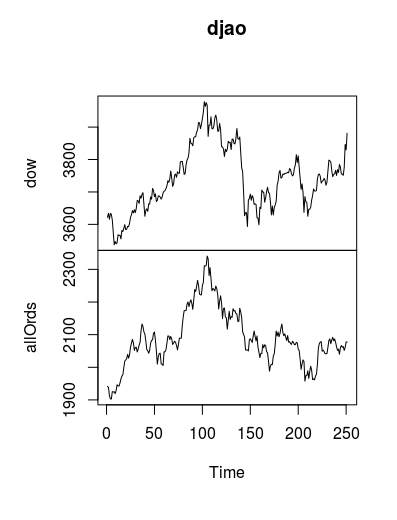
\includegraphics[width=2.00in]{./pics/Rplot}
\end{center}



\end{frame}
%----------------------------------------------------------------------------------------

\begin{frame}[fragile]
\frametitle{Pictures}

Example: Dow Jones and the All Ordinaries Index (Australia)
\newline

See 8.1.R for more details

\begin{center}
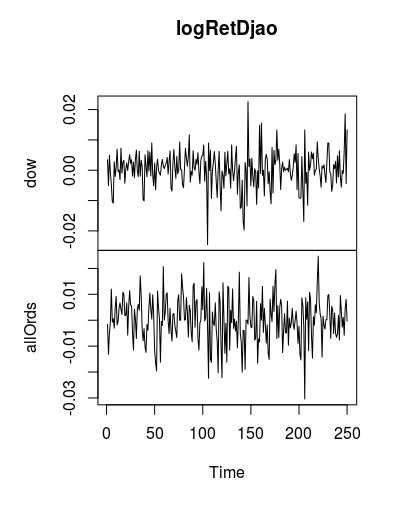
\includegraphics[width=2.00in]{./pics/Rplot01}
\end{center}



\end{frame}
%----------------------------------------------------------------------------------------

\begin{frame}[fragile]
\frametitle{Pictures}

Example: Dow Jones and the All Ordinaries Index (Australia)
\newline

Univariate summaries:

\begin{center}
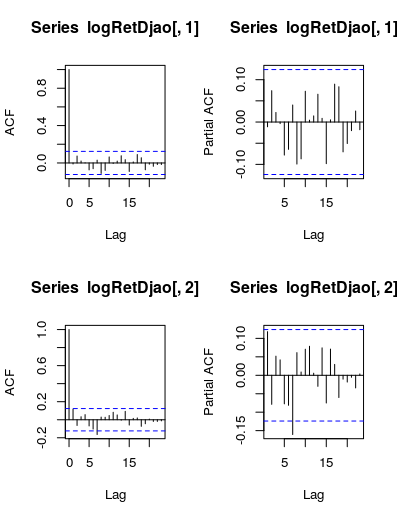
\includegraphics[width=2.00in]{./pics/Rplot02}
\end{center}



\end{frame}

%----------------------------------------------------------------------------------------

\begin{frame}[fragile]
\frametitle{Pictures}

Example: Dow Jones and the All Ordinaries Index (Australia)
\newline

See 8.1.R for more details

\begin{center}
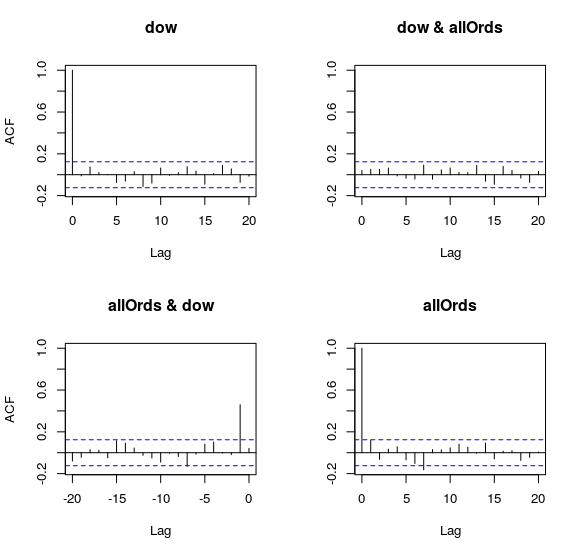
\includegraphics[width=2.50in]{./pics/Rplot03}
\end{center}



\end{frame}

%----------------------------------------------------------------------------------------

\begin{frame}[fragile]
\frametitle{Pictures}

Example: Dow Jones and the All Ordinaries Index (Australia)
\newline

See 8.1.R for more details. $\hat{\rho}_{12}(-1) = .46$


\begin{center}
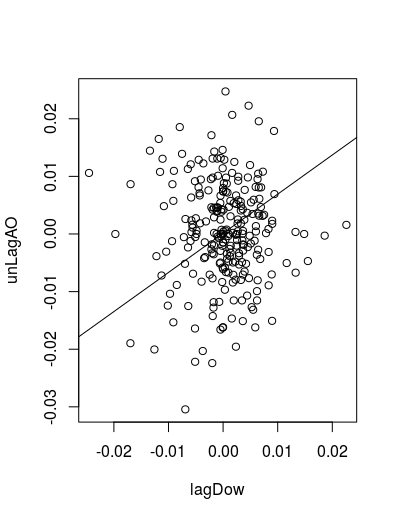
\includegraphics[width=2.00in]{./pics/Rplot04}
\end{center}

\end{frame}




\end{document} 